
\section{PROPOSED FRAMEWORK}
\label{sec:frame}
\begin{figure}
	\centering
	\includegraphics[width=0.9\columnwidth]{flow.png}
	\caption{DCC insertion flow}
	\label{fig:flow}
\end{figure}
\begin{comment}
\begin{figure}
	\centering
	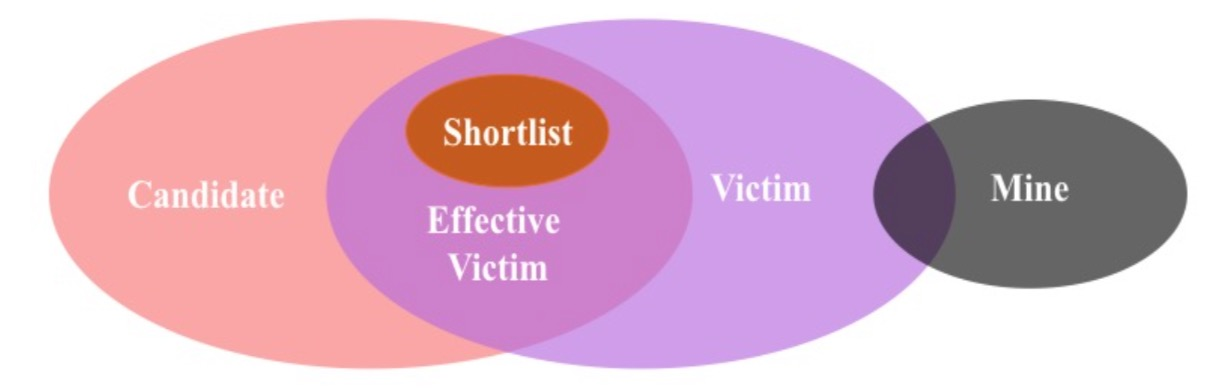
\includegraphics[width=0.9\columnwidth]{pathset.png}
	\caption{Classification of critical paths}
	\label{fig:set}
\end{figure}
\end{comment}
The overall flow of the proposed framework for DCC insertion/deployment is depicted in Figure~\ref{fig:flow}. The proposed framework focuses on the two issues: 
\begin{enumerate}
	\item \textbf{Overhead minimization}: Attacking all critical paths may be infeasible or may increase the used DCC count, which denotes the area overhead of the attack. Thus, the framework must filter/rule out the unpromsing critical paths to make the attack successful and to minimize the DCC count. 
	\item \textbf{Workload variations}: Because users' workload have strong impact on the degradation of logic paths, the proposed framework must consider users' countless operational modes (i.e., workload). To be workload-aware, the problem of selecting target paths to be attacked is transformed to a graph problem, which can be solved using the existing algorithms. 
\end{enumerate}


The section is organized as follows: Section~\ref{sec:frame:cp} discusses the PV-aware methodology of classifying critical path, considering the correlation between PVs and BTI, introduced in Section~\ref{sec:frame:cor}. Section~\ref{sec:frame:workload} details the observation of aging correlation among critical paths. The observation is used in our workload-aware methodology, explained in Section~\ref{sec:frame:mds}, to select target paths to be attacked. Finally, Section~\ref{sec:frame:sat} introduces the SAT-based formulation of DCC deployment.
\subsection{Classification of Critical Paths}
\label{sec:frame:cp}
Given a critical path, the path is classified as one of following three groups: \textit{Shortlist}, \textit{Candidate}, and \textit{Mine}, depending on the lifetime\footnote{The lifetime of a critical path is defined as when the timing violation occurs on the path, in the presence of aging.} distribution\footnote{Given a critical path, a DCC deployment on the associated clock paths results in an individual lifetime value of the critical path. Thus, numerous DCC deployments results in a group of lifetime values, forming the lifetime distribution of the given critical path.} of the critical path, under all possible DCC deployments on the associated clock network. The lifetime distribution of the path is further separated/divided into the three time intervals, which are defined as follows: $[0, n - \varepsilon]$, $[n - \varepsilon, n + \varepsilon]$, and $[n + \varepsilon, \infty]$, where $n$ is the expected lifetime of designs under the proposed HTH attack and $\varepsilon$ is mximum tolerable error. The classification of critical paths can be determined by classifiing/categorizing their lifetime distributions within above intervals. 
\begin{itemize}
	\item \textit{Candidate}: A critical path is defined as a candidate if there exists at least one DCC deployment, which leads the critical path to fail within $[n - \varepsilon, n + \varepsilon]$.
	\item \textit{Mine}: A critical path is defined as a mine if it satisfies the following conditions: ($i$) The path is not a candidate. That is, on the associated clock paths of the critical path, there is no DCC deployment to control the path lifetime within $[n - \varepsilon, n + \varepsilon]$. ($ii$) On the associated clock paths, there exists at least one DCC deployment, which leads the critical path to fail within $[0, n - \varepsilon]$, i.e., it lead the critical path to fail prematurely.
	\item \textit{Shortlist}:  Critical paths in \textit{shortlist} is the subset of \textit{Candidate}, which are selected as target paths to be attacked. Attacking such paths involves deploying DCCs on their associated clock paths.
\end{itemize}
Note that, because of PVs and workload variations, it is impossible to precisely control the lifetime of designs at the expected lifetime $n$, thus, the Trojan attack, controlling the lifetime within $[n-\varepsilon, n+\varepsilon]$ is accepted/desired. Furthermore, the interval $[n - \varepsilon, n + \varepsilon]$ is defined as \textit{desired lifetime interval}. 

To make the classification PV-aware, we conduct Monte-Carlo simulation on the delays of logic paths from statistical perspective. The simulation is performed by imposing extra V\textsubscript{th} offset (i.e., $\Delta V_{th\_pv}$) on each transistor of logic paths. Then, we check the setup-time constraint using Equation~(\ref{eq:setup}), considering the correlation of PVs and BTI, which is introduced in the next subsection. 

\subsection{Path Delay Estimation considering the Correlation between PVs and BTI}
\label{sec:frame:cor}
The correlation is a long-term phenomenon that bridge the V\textsubscript{th} differences among the transistors over a period. Further, a positive/negative V\textsubscript{th} offset leads to a higher/lower fresh V\textsubscript{th}, causing a lower/higher aging speed. Therefore, the gap between high and low V\textsubscript{th} will be gradually converged, letting threshold voltages of transistors, whose fresh ones are different, reach a convergent value. We use a model proposed in~\cite{gomez2016early} to estimate the correlation between fresh V\textsubscript{th} offset (caused by PVs) and BTI effects:
\begin{equation}
	\centering
	\fontsize{9}{9} \selectfont
	\Delta V_{th\_bti} = (1 - S_{v} \cdot \Delta V_{th\_pv})  \cdot A \cdot \alpha^n \cdot t^n
	\label{eq:cor}
\end{equation}
where $\Delta V_{th\_pv}$ is the fresh V\textsubscript{th} offset caused by PVs. $\Delta V_{th\_bti}$ is the BTI-induced V\textsubscript{th} shift, $\alpha$ is the stress duty cycle, $A$ is $3.9 \times 10^{-3} V \cdot s^{-1/_5}$, $n$ is time exponential constant, 0.2 for used technology, and $S_{v}$ is a constant which can be extracted by fitting HSPICE simulation results in 45nm TSMC technology. So far, given a specific $\Delta V_{th\_pv}$ imposed on the V\textsubscript{th} of a transistor, we use Equation~(\ref{eq:cor}) to derive the corresponding $\Delta V_{th\_bti}$, which can be further transformed to BTI-induced delay shift, using the model proposed in~\cite{wang2007efficient}.% the delay shift is linearly proportional to $\Delta V_{th\_bti}$:
\begin{equation}
	\centering
	\fontsize{9}{9} \selectfont
	\Delta t_{p\_aged} = C \cdot \Delta V_{th\_bti}
	\label{eq:vtodelay}
\end{equation}	
where $\Delta t_{p\_aged}$ is BTI-induced shift of propagation delay, and $C$ is a constant and is fitted to 0.5 after SPICE simulation. Further, the Equation~(\ref{eq:vtodelay}) is modified as following Equation~(\ref{eq:vtodelay2}) to account for the conversion from $\Delta V_{th\_pv}$ to intrinsic delay shift. 
\begin{equation}
	\centering
	\fontsize{9}{9} \selectfont
	\Delta t_{p\_intrinsic} = C \cdot \Delta V_{th\_pv}
	\label{eq:vtodelay2}
\end{equation}	
where $\Delta t_{p\_intrinsic}$ is the propagation delay shift caused by $\Delta V_{th\_pv}$. Up to now, a model is built to convert a given specific $\Delta V_{th\_pv}$ to corresponding $\Delta t_{p\_aged}$ and $\Delta t_{p\_intrinsic}$. The model is not only used in the classification of critical paths, but also used in Section~\ref{sec:lt_estimation} while estimating the intervals of Monte-Carlo instances of attacked designs. 
%------- Shortlist selection --------------------------------------------------------------------------------------------------
\subsection{Selection of Target Paths (Shortlist) to be attacked considering Workload Variations}
\label{sec:frame:workload}
\begin{figure}
	\centering
	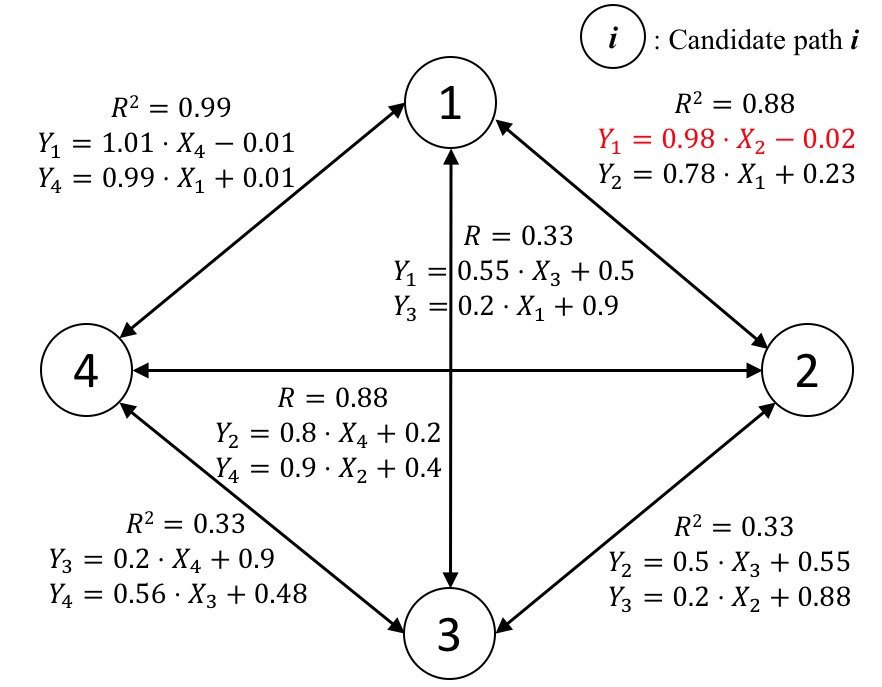
\includegraphics[width=0.8\columnwidth]{graph.png}
	\caption{Example of graph used in choosing targets}
	\label{fig:graph}
\end{figure}

The uncertainty of user-dependent operational modes (e.g., watching video, playing games) can influence/vary the aging behavior of logic paths. Therefore, we should ensure that the attack will succeed under any operational mode. We assert the following assumption, which is also used in Section~\ref{sec:lt_estimation} to estimate the lifetime interval of attacked designs:

\noindent \textbf{\uline{Assumption: Every operational mode causes at least one candidate path to undergo severe aging.}}

In other words, no matter how users operate the design, at least one candidate path undergoes severe aging. Moreover, given a path, if an operational mode leads the path to undergo severe aging, the operational mode is defined as the \textit{critical operational mode} of the path:

\noindent \textbf{\uline{Definition: An operational mode, which leads the path to undergo severe aging, is defined as a critical operational mode of the path.}}

This way, the following corollary can be obtained:

\noindent \textbf{\uline{Corollary: The union of critical operational modes of all candidate paths is equivalent to the universal set of operational modes.}}

Therefore, attacking all candidate paths is a na\"ive method to guarantee the successful attack regardless of the users' workload variations, while it is very costly and may be impossible. 
However, when we attack the fraction of candidate paths, it is still possible to make the attack successful if we consider the correlation of aging behaviors among critical paths. Specifically speaking, we observe that the aging behaviors of many paths are highly correlated. For instance, given two critical paths A and B, suppose that A and B are highly correlated in terms of their aging behaviors, the critical operational mode of A, $O_{A}$, must lead A to age severely, according to the aforementioned definition. In addition, $O_{A}$ also leads B to a similar level of aging because A and B age closely/similarly. Consequently, even if we simply attack path $A$, both $O_{A}$ and  $O_{B}$ can make the attack successful. In short, we can simply attack one out of those highly correlated paths to cover multiple operational modes. This property helps reduce the count of targeted paths to be attacked.%considered/formulated.

\subsection{Selection of Target Paths using MDS (Minimum Dominating Set)}
\label{sec:frame:mds}
Based on the aforementioned property of aging correlation of paths, a directed graph (also known as digraph) is constructed as shown in Figure~\ref{fig:graph}, where vertices represent candidates and arcs (i.e., directed edges) are correlation coefficients ($R^2$) and linear regression equations between each pair of vertices. Each arc has a regression equation, where $X_{i}$ denotes the severe aging rate of path $i$, $Y_{j}$ denotes the aging rate of path $j$ predicted based on the linear regression equation and the other coefficients are obtained by running functional simulation. The exact value of $X_{i}$ can be derived by the following predictive model presented in \cite{wang2007efficient}:
\begin{equation}
	\fontsize{8}{8} \selectfont
	A \cdot \alpha^n \cdot t^n 
	\label{eq:worst}
\end{equation}
where $A$ and $n$ are fitted constants, $\alpha$ denotes the stress duty cycle, and $t$ denotes time (unit is second). $\alpha$ is usually set to 0.5. $A$ and $n$ are fitted as 0.0039 and 0.2, respectively, after SPICE simulation.

Consider the red equation in Figure~\ref{fig:graph}:
\begin{equation}
	\centering
	\fontsize{8}{8} \selectfont
	Y_{1} = 0.98 \cdot X_{2} - 0.02
\end{equation}
where $X_{2}$ is aging rate of vertex/path 2 and $Y_{1}$ is the aging rate of vertex/path 1, which can be predicted as 0.98 multiplied by $X_{2}$ minus 0.02.
Moreover, after the graph is constructed, it is further simplified by removing some arcs, which indicate the weak aging correlation between pairs of paths/vertices.

We aim to select the minimum-sized of targets, that is, the minimum dominating set in the digraph to cover all candidate paths. Such the proposed Trojan attack is capable of considering all users' operational modes based on the corollary. This problem is transformed to the classical digraph problem, \textbf{Minimum Dominating Set (MDS)}, which can be solved using the existing algorithms proposed in \cite{ore1962theory}\cite{natarajan1978optimum}. The MDS problem is defined as follow:

\textit{On digraph $G = (V, E)$, find a minimum-sized set of vertices $S \subseteq V$ such that $\forall y \notin S$, $\exists x \in S$, there exists an arc from $x$ to $y$. And we say that $y$ is dominated by $x$}.

%Therefore, after observing the relationship among aging of paths, we find that the aging behaviors of many paths are highly correlated. If several paths are highly correlated in terms of aging behavior, one operational mode can lead all of them to age to a similar extent. Thus, we can simply attack one out of those highly correlated paths to cover multiple operational modes. For example, given two critical paths $A$ and $B$. Their critical operational modes are $O_{A}$ and $O_{B}$, respectively. Assume that $A$ and $B$ are highly correlated in terms of aging behavior. Because $A$ and $B$ age similarly/closely, $O_{A}$ causes $A$ to age in the severe and also causes $B$ to age severely. Consequently, even if we simply attack path $A$, not only $O_{A}$ but also $O_{B}$ can make the attack successful (i.e., control the lifetime of path $A$ within the interval [$n - \varepsilon, n + \varepsilon$]). This property helps reduce the count of targeted paths to be considered/formulated. 

%------- SAT  --------------------------------------------------------------------------------------------------
\subsection{SAT-based Problem Formulation and Encoding for DCC Deployment}
\label{sec:frame:sat}
\begin{comment}
	\begin{figure*}[!ht]
    	\centering
    	\subfigure[A DCC deployment leads path $p$ to fail prematurely]{
    		\label{fig:sub:upper}
        		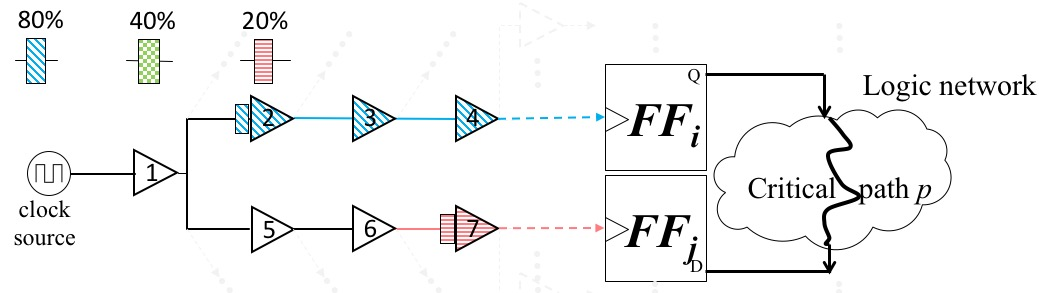
\includegraphics[width=0.9\columnwidth]{upper.png}
    	}
   	\hspace{0.1cm}
    	\subfigure[A DCC deployment leads path $p$ to fail post-maturely]{
    		\label{fig:sub:lower}
        		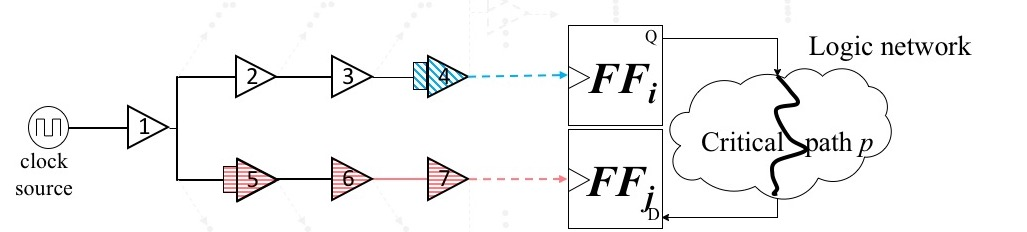
\includegraphics[width=0.92\columnwidth]{lower.png}
    	}
    	\caption{Illustrative example for the proposed framework based on DCC deployment/insertion}
    	\label{fig:en}
	\end{figure*}
\end{comment}
\begin{figure}
    	\centering
        	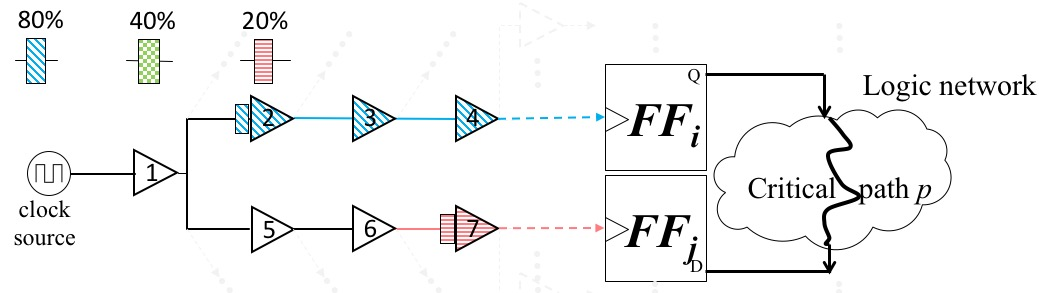
\includegraphics[width=0.9\columnwidth]{upper.png}
       	\caption{A DCC deployment leads path $p$ to fail prematurely}
    	\label{fig:sec:prefail}
\end{figure}
After the shortlist (i.e., target paths to be attacked) is determined using existing MDS algorithms, the problem of DCC deployment is formulated as a \textbf{Boolean satisfiability (SAT)} problem. The authors of~\cite{wu2018maui} also use the SAT-based approach to determine the DCC deployment in the existing clock tree, while they aim to improve aging tolerance of designs. The key of our framework is to represent the problem in \textit{conjunctive normal form} (CNF). A CNF representation is a conjunction of one or more clauses, where each clause is a disjunction of one or more Boolean variables. Thus, DCC deployment/insertion needs to be encoded into Boolean representation before being transformed into a SAT-based formulation. Assume that a total of 3 types of DCCs can be chosen (i.e., 20\%, 40\%, and 80\% DCCs). Including the DCC-free case (i.e., no DCC is inserted), there are 4 possibilities of DCC insertion for each clock buffer. Given a clock buffer $p$, the four possibilities of DCC insertion at the input of buffer $p$ can be encoded using the  following two Boolean variables $B_{p,2}$ and $B_{p,1}$:

{\small
\begin{tabular}{ c c c }
   & DCC type & $\left\{B_{p,2},B_{p,1}\right\}$ \\
  (1)\quad & None & \{0,0\} \\
  (2)\quad & 20\% &  \{0,1\} \\
  (3)\quad & 40\% &  \{1,0\} \\
  (4)\quad & 80\% &  \{1,1\} \\
\end{tabular}}

To control the lifetime of designs within $[n - \varepsilon, n + \varepsilon]$, timing constraints of DCC deployments are formulated in the SAT-based problem. The formulations of timing constraints depend on the classification of critical paths.
\begin{enumerate}
	\item Paths in the shortlist: The lifetime of shortlist paths dominate the lifetime of attacked designs. To control the lifetime of shortlist paths within $[n - \varepsilon, n + \varepsilon]$, on their associated clock paths, we formulate all DCC deployments, which lead the path to fail prematurely or post-maturely (i.e., within $[ 0, n - \varepsilon]$ or within $[ n + \varepsilon, \infty]$), such that the SAT solver will not output the corresponding deployment in the result if the CNF is satisfiable.
	\item Other paths (paths not in the shortlist): While attacking shortlist paths, the DCC deployment may cause the premature failure of other paths excluded in shortlist, because they have significant share of the common sub-paths, and give rise to the proposed Trojan attack premature and inaccurate. Thus, to allow the attack effectively and avoid picking up the unsuitable paths to compromise, we formulate all DCC deployments, which lead the paths to fail prematurely (i.e., within $[ 0, n - \varepsilon]$), such that the SAT solver will not output the corresponding deployment in the result if the CNF is satisfiable.
\end{enumerate}

Consider the example in Figure~\ref{fig:sec:prefail}, where the 80\% and 20\% DCCs are inserted at the inputs of buffer 2 and 7, respectively and assume that the critical path $p$ is in shortlist. If the DCC deployment will lead the path $p$ to fail prematurely (i.e., path fail within $[ 0, n - \varepsilon]$), then the following clause
\begin{gather*}
	\fontsize{9}{7} \selectfont
	\mbox{($A_{1} \lor A_{0} \lor \neg B_{1} \lor B_{0} \lor C_{1} \lor C_{0}$) } 
\end{gather*}
will be generated and added into the final CNF, such that the solver will not output the corresponding DCC deployment in the result if the CNF is satisfiable.

For SAT-based formulation, the problem of DCC deployment is transformed into CNF clauses, and they can be solved by SAT solver such as MiniSat. Finally, we can find the locations and types of inserted DCCs by decoding the output returned from the solver.



